\documentclass[12pt,twocolumn,letterpaper]{article}

\usepackage{cvpr}
\usepackage{times}
\usepackage{epsfig}
\usepackage{graphicx}
\usepackage{amsmath}
\usepackage{amssymb}
\usepackage[breaklinks=true,bookmarks=false]{hyperref}
\usepackage{gensymb}
\usepackage{subcaption}

\cvprfinalcopy

\def\httilde{\mbox{\tt\raisebox{-.5ex}{\symbol{126}}}}


\setcounter{page}{1}
\begin{document}

\title{3D Perspective Effects on a Smart Phone}

\author{Jai Prakash\\
Carnegie Mellon University\\
Master of Science in Computer Vision\\
{\tt\small jprakash@andrew.cmu.edu}
\and
Jennifer Lake\\
Carnegie Mellon University\\
Master of Science in Computer Vision\\
{\tt\small jelake@andrew.cmu.edu}
}

\maketitle

\begin{abstract}
In this project, we aim to create a 3D perspective transformation on a smart phone screen that will give the illusion of screen having depth.  The user should feel as if they are looking into a long hallway, were objects can appear deeper and deeper into the hall. This is achieved by finding the three-dimensional vector between the user’s face and the center of the phone.  This was achieved by tracking the user’s face using the front-facing camera.  We also explored integrating this method with the smart phone's Internal Measurement Unit (IMU) in order to estimate the smart phone orientation. In both methods, Kalman filtering was used in order to create a more reliable vector prediction.
\end{abstract}

\section{Introduction}
\subsection{Motivation}
As mobile phones have evolved over the last twenty years, many of the major milestones have been in display improvements. Mobile phones have gone from very small, simple displays to larger and more colorful displays.  At the forefront of this evolution, there is a growing trend of three-dimensional displays. 

There are several benefits to having more 3D-like displays.  3D-like displays may help users interact with User Interfaces in a more intuitive way, such as using the phone movement itself as a command.  This can help when using the phones when wearing gloves, which do not allow the use of the touch screen.  In addition, 3D-like displays may help users navigate using 3D maps, which are more representative of the surroundings in urban areas. Finally, 3D-like displays would be a major boost to the gaming industry, which constantly strives to make more and more realistic games.  With perspective effects that mimic real-world perspective effects, the user would experience a more immersive gaming experience.

The holy grail of 3D perspective transforms is to be able to provide augmented reality to the user.  This would allow the user to use their smart phone to interact with the world around them in an intuitive manner, such as in figure 1.  We hope that some of the work in this project, may help in future projects striving towards this goal.

\begin{figure}
\centering
\begin{subfigure}{0.22\textwidth}
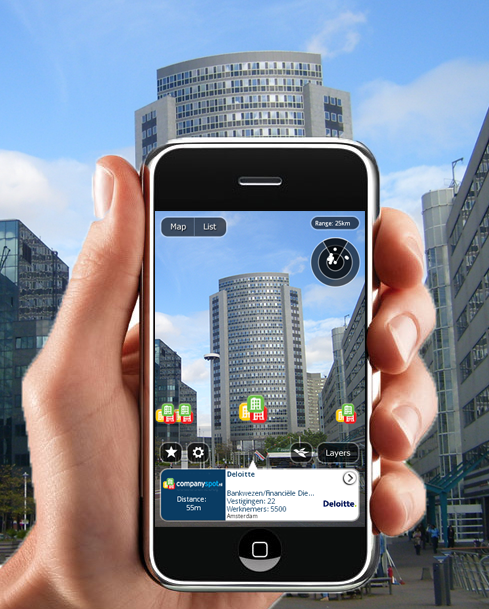
\includegraphics[height=35 mm]{AR_now}
\end{subfigure}
\begin{subfigure}{0.22\textwidth}
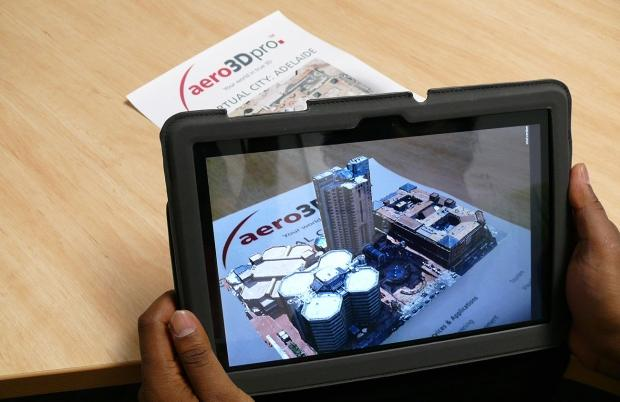
\includegraphics[height=25 mm]{AR_now1}
\end{subfigure}
\caption{Augemented reality in present smartphones}
\label{fig:arnow}
\end{figure}

\subsection{Background}

The change in appearance of an object when viewed from multiple viewpoints is known as parallax \cite{Szeliski}.  Parallax occurs due to the shift in perspective.  An example of the parallax effect is shown below \cite{Wikipedia}.

\begin{figure}[!htbp]
\centering
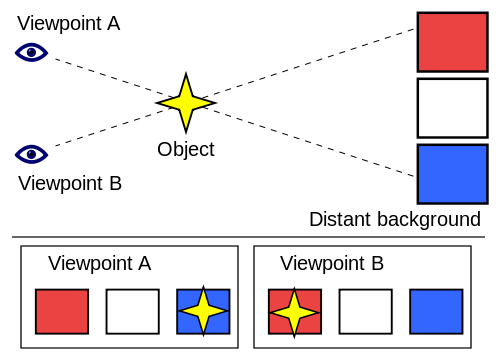
\includegraphics[height=30 mm]{parallax.png}
\caption{An example of the parallax effect.  The top of the figure shows the scene from above.  The bottom of the figure shows the views from each viewpoint.}
\end{figure}

There are three types of parallax effects: negative, zero, and positive parallax (figure 2) \cite{CSU}.  

\begin{figure}[!htbp]
\centering
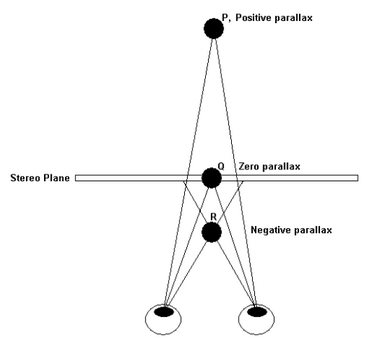
\includegraphics[height=35 mm]{NegPosParallax.png}
\caption{Example of positive, zero, and negative parallax}
\end{figure}

Positive parallax occurs when the user gets the impression of looking through the screen plane and this effect will be the focus of this project.  Negative parallax occurs when the user get the impression that objects are floating above the user screen and this effect will not be addressed in this project.  Zero parallax is the impression that the object lies on the screen and this conventional way of viewing objects on a screen.

\subsection{Related Work}
The trend of introducing of positive parallax effects into smart phones has been growing in the last few years.  In 2013, Apple introduced the positive parallax effect on their line of iPhones, which allows for a 3D-like feeling, by changing the position of the background wallpaper according to the orientation of the smart phone \cite{BusinessInsider}.  A year later, the Amazon Fire Phone introduced a full positive parallax effect, which was branded as "Dynamic Perspective" \cite{DigitalTrends}.  It is this type of effect that we aim to create in this project however, unlike the Amazon Fire Phone, we will be implementing this effect on simpler, standard smart phone hardware.

Prior to the growing trend in parallax effects in smart phones, the Microsoft Kinect was to estimate a person's pose and using that information, render a parallax effect on a television screen.  One interesting example of this is the Virtual Window, which has a television behind a false window and the landscape on the television changes based on the perspective of the user.  One major constraint of this type of system is that the perspective change only works for one user at a time.

In the future, we expect parallax effects to lead to Augemented Reality for smart phones.  This could allow users to seamlessly interact with the surrounding environment and could lead to new uses for smart phones.

\subsubsection{Virtual Window}
The Virtual Window works by using a Microsoft Kinect sensor, which projects a light pattern onto the user and uses an RGB-D camera to find the pose and 3-dimensional pose of the user \cite{Winscape}.  Using this information, the position of the user's head and eyes can be located using built-in tools in the Kinect API.  A high-resolution, high-quality image of an outdoor scene is then moved in order to simulate that the screen is in fact a window.  The image only needs to be shifted to the appropriate location because the images are taken from far away (see figure 4).

\begin{figure}[!htbp]
\centering
\begin{subfigure}{0.22\textwidth}
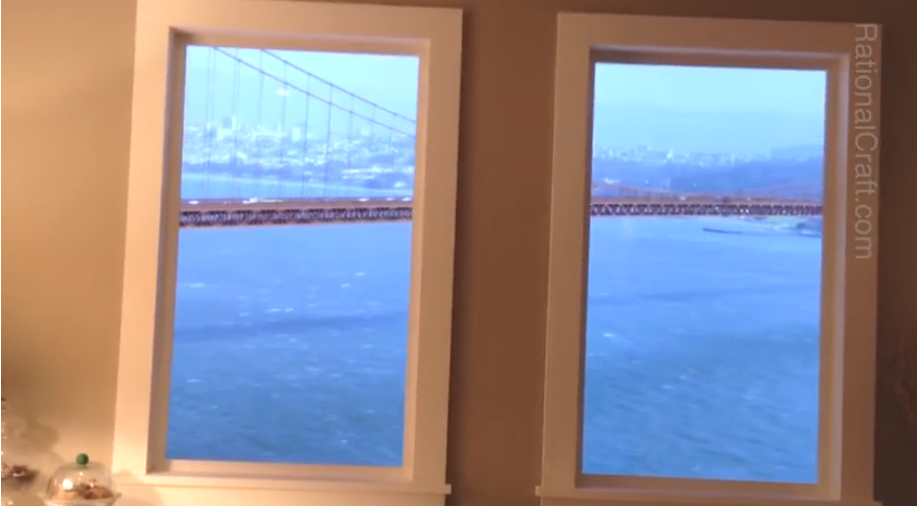
\includegraphics[width = 35 mm]{win1.png}
\end{subfigure}
\begin{subfigure}{0.22\textwidth}
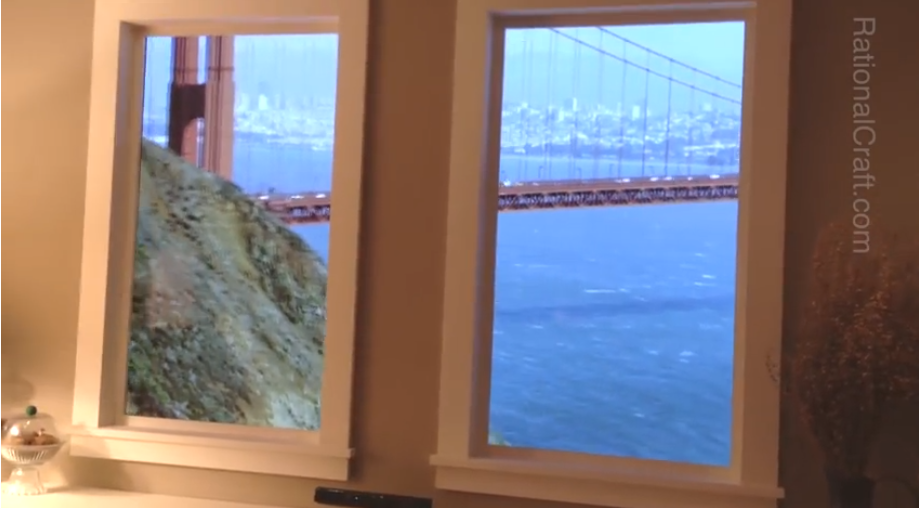
\includegraphics[width = 35 mm]{win2.png}
\end{subfigure}
\caption{Virtual Window from two different perspectives}
\end{figure}

\subsubsection{Amazon Fire Phone}
The Amazon Fire Phone uses four, front-facing camera's with wide 120 \degree viewing angles \cite{TechCrunch}.  This allows for at least two cameras to be able to locate the user's face, regardless of how the phone is held.  The face tracking works in low light as well, due to infrared light being used to illuminate the user's face.  By tracking the user's face, the vector between the phone and the user can be approximated and thereby the correct perspective transform can be computed and displayed.

\begin{figure}[!htbp]
\centering
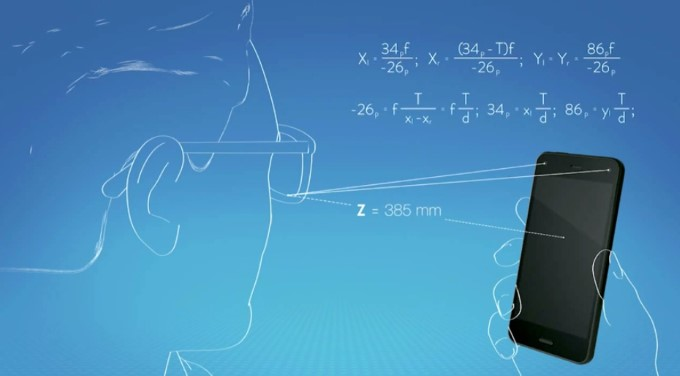
\includegraphics[height=35 mm]{dp.jpg}
\caption{Example of Amazon Fire Phone's Dynamic Perspective}
\end{figure}

\subsubsection{Augmented Reality}

The ultimate goal of estimating a phone's orientation with respect to the user is to be able to implement Augmented Reality (AR) into smart phones. The smart phone Augmented Reality can broadly be classified into two types:
\begin{itemize}
\item \textbf{Indirect AR} Figure \ref{fig:arnow} shows augmented reality applications in current smart phones. This gives the user a video see-through experience, as the view is from the camera's perspective.
\item \textbf{Direct AR} These are the systems that give a perspective from user's point of view and hence give more immersive experience than indirect AR system. The Microsoft Hololens and meta-glasses (Figure \ref{fig:directar}) are examples of direct AR systems. 
\end{itemize}


\begin{figure}[!htbp]
\centering
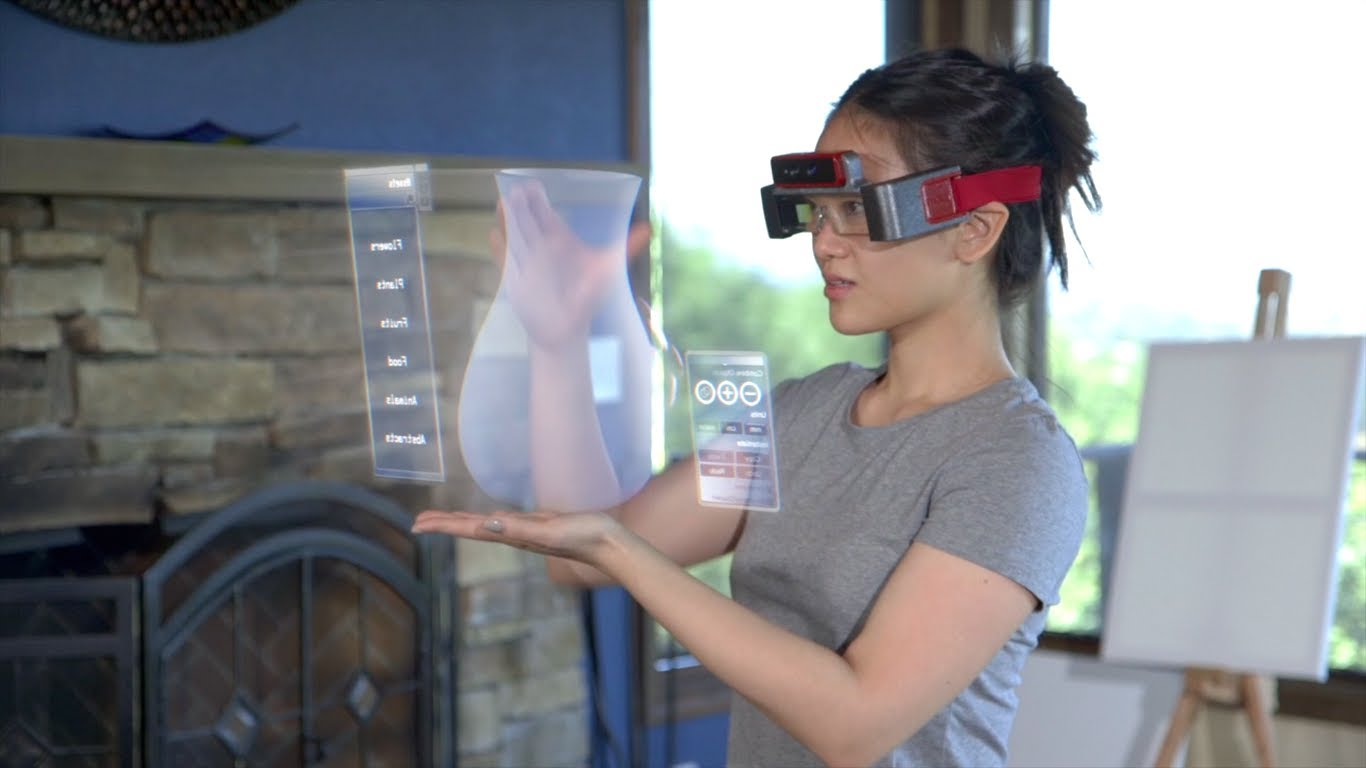
\includegraphics[height=30 mm]{mata}
\caption{Direct AR from Meta-glasses}
\label{fig:directar}
\end{figure}

The current direct AR systems are generally bulky and requires user to wear special glasses to use them. However, a direct AR system can be achieved in smart phones and tablets by using digital transparency \cite{jai}. Digital transparency system is shown in Figure \ref{fig:digitaltransparency}. This system tracks the eyes of the user and finds the angle which the tablet subtends at user's eye and crops the rear camera preview to the same angle to create a virtually transparent interface. This system gives a method to achieve direct AR on smart phones and tablets, thereby giving a more immersive \textbf{glass-see-through} experience than the conventional \textbf{video-see-through} experience.

\begin{figure}[!htbp]
\centering
\begin{subfigure}{0.22\textwidth}
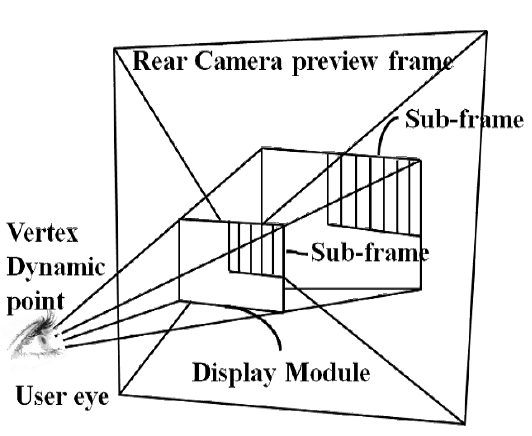
\includegraphics[height=30 mm]{transparenttablet}
\end{subfigure}
\begin{subfigure}{0.22\textwidth}
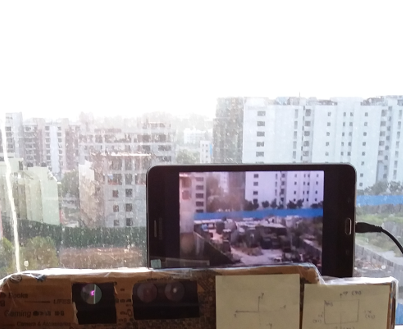
\includegraphics[height=30 mm]{transparenttablet1}
\end{subfigure}
\caption{Digital transparency using Kinect on Android tablet}
\label{fig:digitaltransparency}
\end{figure}

This method uses a Kinect sensor to track the accurate 3D position of the user with respect to tablet. The Kinect sensor makes the system bulkier and difficult to use in smart phones. So, in this project we are addressing another method to achieve digital transparency using just the front facing camera and attempting to integrate the inertial sensors. A complete hands-free digital transparency system is out of scope of this project. The main concentration is on creating a positive parallax effect which responds to the user's position with respect to the tablet.

\section{Method}
\begin{figure}[!htbp]
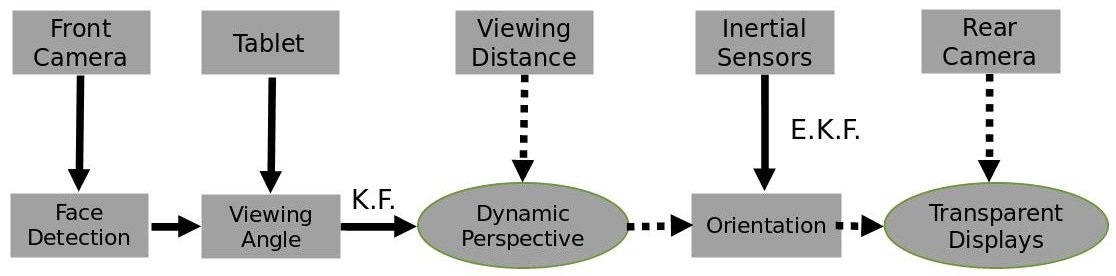
\includegraphics[scale=0.21]{block}
\caption{Block diagram of system}
\label{fig:blockdia}
\end{figure}

Creating a positive parallax effect involves finding the viewing angle of the user and rendering the graphical object depending on position of the user. This might involve one of three scenarios:
\begin{itemize}
\item Tablet is static and user moves
\item Tablet moves and user is static
\item Both tablet and the user can move
\end{itemize}

In order to limit the scope of the project, we have also placed a number of restrictions on how this systems is to be used.  We also assume the following restrictions:

\begin{itemize}
\item There are no drastic lighting changes
\item The user is not walking or running
\item The user is standing or sitting on a stationary surface.
\item The user and the tablet are moving smoothly and slowly
\item The tablet is held at a constant distance from the user's face.
\item There is only one user and the user is always in view of the front camera.
\item There are no other faces in the view of the front camera
\item The user is looking at the camera or very close to it
\item The user is an arm's length or less from the camera
\item The user's face is the primary object in the view of the camera
\end{itemize}

To find the motion and orientation of the phone, on-board inertial sensors can be deployed to find the orientation of the phone. A study on sensor fusion has been made to find the orientation of the phone.

The block diagram of the system is shown in the figure  \ref{fig:blockdia}. Solid arrow shows the algorithms implemented for this project. The dotted arrow parts are yet to be figured out to build a full-fledged digital transparency system. However, the main focus is only on creating the positive parallax effect.

To create this effect, we need to first track the position of user with respect to the tablet. In this project we assume that the distance of the eye from tablet is fixed (approximately 45-50 cm). This assumption fails to address the scale factor in dynamic perspective. Therefore we don't get zoom-in and zoom-out effect as we move forward and backward. Since the distance from the tablet is assumed to be constant, we use the viewing angle to render the user interface (UI) in 3D. The following sections describe the exact methods used in each step.

\subsection{3D Geometry of Problem}
In order to render a positive parallax effect, we must estimate the vector between the user and the phone, as shown in figure \ref{fig:vectors}.

\begin{figure}[!htbp]
\centering
\begin{subfigure}{0.22\textwidth}
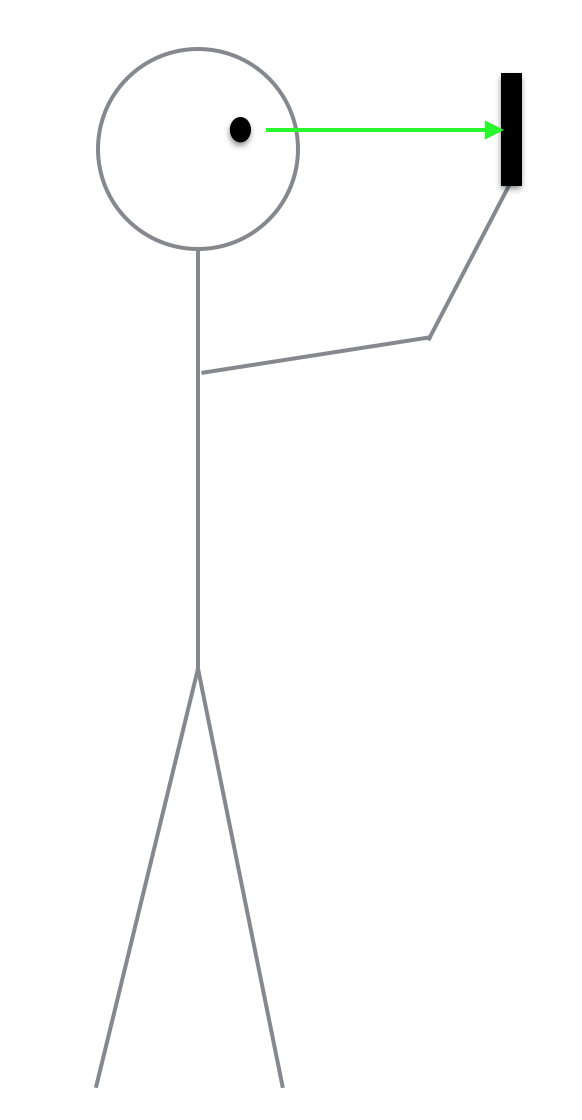
\includegraphics[height=30 mm]{vector1}
\end{subfigure}
\begin{subfigure}{0.22\textwidth}
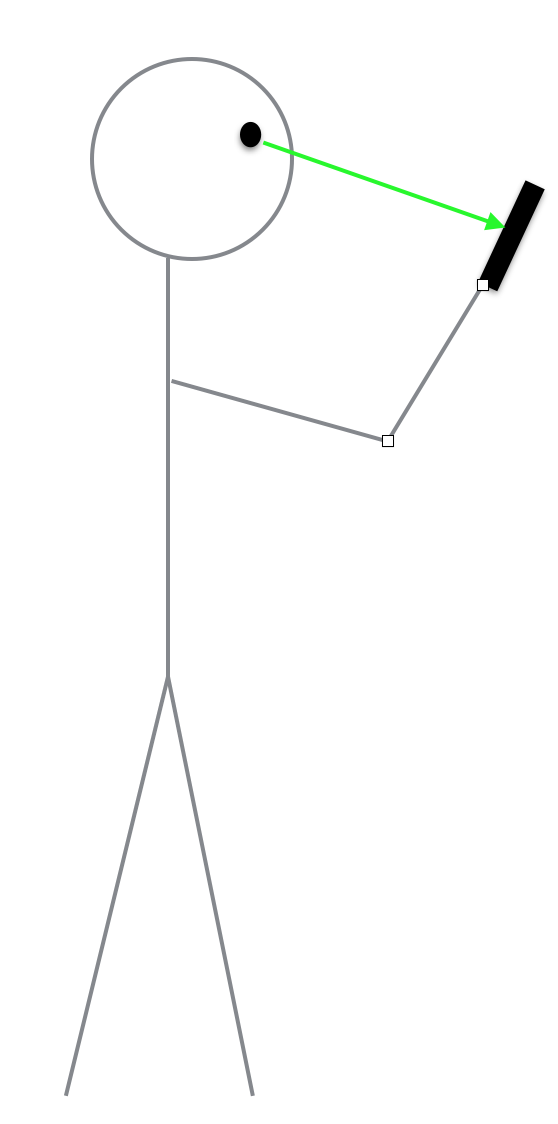
\includegraphics[height=30 mm]{vector2}
\end{subfigure}
\caption{Example of vectors to be found}
\label{fig:vectors}
\end{figure}

Normally, a user will hold a smart phone orthogonally to the vector between the user's eye and the principle point of the camera (figure \ref{fig:orthogonal}).  This is a natural position of the screen, since it is easiest to view from this angle and does not strain the eyes.   

\begin{figure}[!htbp]
\centering
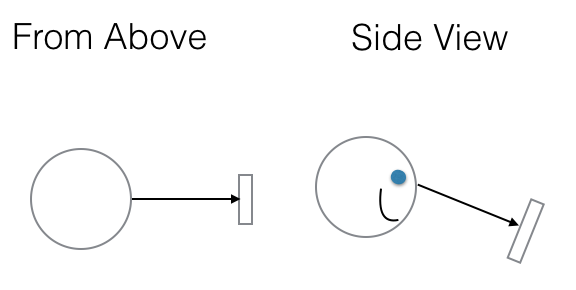
\includegraphics[height=30 mm]{conventional.png}
\caption{Conventional way of holding a smart phone}
\label{fig:orthogonal}
\end{figure}

However, it is possible for the user to hold the smart phone in an unconventional matter, such as in figure \ref{fig:unconventional}.

\begin{figure}[!htbp]
\centering
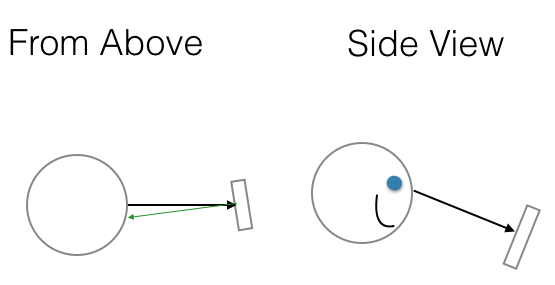
\includegraphics[height=30 mm]{unconventional.png}
\caption{Unconventional way of holding a smart phone.}
\label{fig:unconventional}
\end{figure}

     -Jenna: finish this

\subsection{Finding viewing angle of user}
Since all the coordinates are in image frame of reference, the angle can be found by using the following equations. 
\begin{equation}
\theta_x = tan^{-1} \left( \frac{x_f - \frac{W}{2}}{f_x} \right)
\label{eqn:thetax}
\end{equation}
\begin{equation}
\theta_y = tan^{-1} \left( \frac{y_f - \frac{H}{2}}{f_y} \right)
\label{eqn:thetay}
\end{equation}

In equation \ref{eqn:thetax} and \ref{eqn:thetay}, $(x_f, y_f)$ is the location of the centroid of the user's face. Image size is $W \times H$. $f_x$ and $f_y$ are the focal length of the camera in pixels.

\begin{figure}[!htbp]
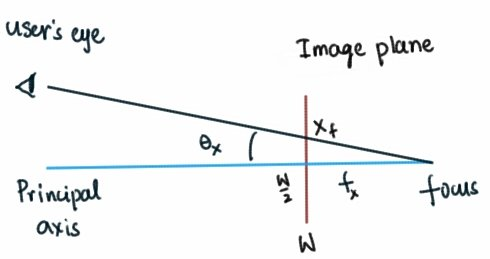
\includegraphics[scale=0.5]{view_angle}
\caption{The viewing angle of the user with respect to front camera on smart phone}
\label{fig:viewangle}
\end{figure}

Figure \ref{fig:viewangle} shows the viewing angle of the user. The view angle is the angle subtended by the user's position with the principal axis of the camera. The focal length of the camera is found by using camera calibration in OpenCV \cite{calibration}. 

    -Jai: Include equations from reference


\subsection{Face Detection}
The Viola-Jones algorithm was used for face detection because it is robust and fast \cite{Viola-Jones}.  The Viola-Jones algorithm has four main steps:

\begin{enumerate}
\item Compute Haar Features
\item Compute Integral Image
\item Use AdaBoost to Train Classifier
\item Cascade Classifiers
\end{enumerate}

In the first step, Haar features are computed.  Haar features represent simple structure present in human faces, such as darker eyes and lighter cheeks or a lighter nose and darker eyes.  These features are calculated at different orientations. An example of Haar features can be found in figure \ref{fig:Haar}.

\begin{figure}[!htbp]
\centering
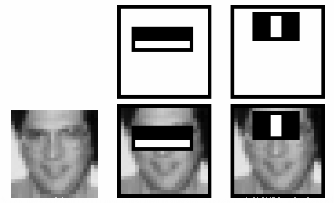
\includegraphics[scale=0.5]{haar}
\caption{An example of Haar features}
\label{fig:Haar}
\end{figure}

The integral image is then computed by summing the value of a pixel and all pixels to the left and above it.  This can be done in one pass if the integral image is calculated from the origin outward using equation \ref{eqn:integral}. This is done so that the Haar calculations, which are defined in equation \ref{eqn:haar} can be completed quickly.

\begin{multline}
\label{eqn:integral}
I(x,y) =  i(x,y) + I(x-1,y) 
\\+ I(x, y-1) - I(x-1, y-1)
\end{multline}


\textbf{\begin{equation}
\label{eqn:haar}
score = \sum{black pixels} - \sum{white pixels}
\end{equation}}

    -Jenna : finish this
    
\subsection{Inertial Measurement Unit}
An Inertial Measurement Unit (IMU), is a sensor that features a triad of accelerometers and a triad of gyroscopes \cite{Graves}.  In cell phones, the IMU also typically features a magnetometer. 
   
   -Jenna : finish this 
    
\subsection{Kalman Filter}
    -Jai : Include equations
\subsection{Extended Kalman Filter}
    -Jenna : Include Equations
\section{Experiments}
\subsection{Image Geometry Experiments}
 - Jai: put results here / how it was done
\subsection{Camera Calibration}

The camera calibration matrix is returned as
\begin{equation}
K = \begin{bmatrix}
f_x & \alpha_x & c_x\\
0 & f_y &  c_y\\
0 & 0 & 1
\end{bmatrix} = \begin{bmatrix}
145 & 0 & 930\\
 0 &145 & 601\\
0 & 0 & 1
\end{bmatrix}
\end{equation}

The value of the focal length is in terms of the pixels. The resolution of the camera is 1920x1280, and the principal axis seems to be almost at the center of the image.
\subsection{IMU Experiments}
    -Jenna: put results here and how much it sucked
\section{Conclusions}
    -Both: wrap it up, future work if room is needed
    
{\small{
\begin{thebibliography}{15}

\bibitem{Szeliski}
Szeliski, Richard. \textit{Computer Vision: Algorithms and Applications}. 1st ed. London: Springer-Verlag, 2010. Print.

\bibitem{Wikipedia}
\textit{Parallax Example}. Digital image. \textit{Wikipedia}. Wikimedia, 31 May 2006. Web. 15 Dec. 2015.

\bibitem{CSU}
Positive vs. Negative Parallax. Digital image. \textit{CSE 621 Contemporary Computer Graphics}. California State University, San Bernadina, n.d. Web. 15 Dec. 2015.

\bibitem{BusinessInsider}
Yarow, Jay. "Here's Why Apple Made That Motion-Effect For The Background Of The New IPhone Software." Business Insider. Business Insider, Inc, 25 Sept. 2013. Web. 11 Dec. 2015.

\bibitem{DigitalTrends}
Pelegrin, Williams. "Why Isn’t the Fire Phone Truly 3D? Amazon’s ‘Dynamic Perspective’ Tech Explained." \textit{Digital Trends}. Digital Trends, 18 June 2014. Web. 11 Dec. 2015.

\bibitem{Winscape}
Sevilla, Beth. "Winscape." \textit{Winscape}. Rational Craft, n.d. Web. 14 Dec. 2015.

\bibitem{TechCrunch}
Crook, Jordan. "Amazon’s Fire Phone Uses Depth And 3D Effects To Stand Out." \textit{TechCrunch}. TechCrunch, 18 June 2014. Web. 14 Dec. 2015.

\bibitem{jai}
Prakash, Jai, and Ajay Vijayvargiya. A Method for Obtaining Digital Transparency in Electronic Devices. Samsung, assignee. Patent 4506/CHE/2014. 16 Sept. 2012. Print.

\bibitem{Engaget}
Alvarez, Edgar. Dynamic Perspective. Digital image. \textit{Engaget}. AOL, 8 June 2014. Web. 15 Dec. 2015.

\bibitem{kalman}
 Kalman, R. E. "A New Approach to Linear Filtering and Prediction Problems". \textit{Journal of Basic Engineering, 1960}

\bibitem{Viola-Jones}
Viola, Paul, and Michael J. Jones. "Robust Real-Time Face Detection." \textit{International Journal of Computer Vision} 57.2 (2004): 137-54. \textit{ProQuest}. Web. 15 Dec. 2015.

\bibitem{calibration}
"Camera Calibration With OpenCV." \textit{OpenCV 3.0.0 Documentation}. Itseez, 10 Nov. 2014. Web. 15 Dec. 2015.  \url{http://docs.opencv.org/3.0-beta/doc/tutorials/calib3d/camera_calibration/camera_calibration.html}.

%to be used

\bibitem{Graves}
Graves, Joe. "Design And Control Of A Vehicle For Neutral Buoyancy Simulation Of Space Operations." Thesis. University of Maryland, 1997. Print.

\bibitem{ArsTechnica}
Cunningham, Andrew. "IPhone 6 and 6 Plus: In Deep with Apple’s Thinnest Phones." \textit{Ars Technica}. Conde Nast, 22 Sept. 2014. Web. 14 Dec. 2015.

\bibitem{Gizmodo}
Aguilar, Mario. "Here's Why the IPhone 5S Accelerometer Is So Screwed Up." \textit{Gizmodo}. Gawker Media, 16 Oct. 2013. Web. 14 Dec. 2015.

\bibitem{Quan}
Quan, Wei. \textit{INS/CNS/GNSS Integrated Navigation Technology}. Heidelberg: Springer, 2015. \textit{Springer Link}. Springer. Web. 14 Dec. 2015.

\endgroup
\end{document}